
\section{Der Serresche Dualitätssatz}
\label{sec:serre}

\begin{defin}
  \label{def:res}
  Sei $X$ eine kompakte Riemannsche Fläche. Nach \cite[Satz 15.14]{For} ist
  \[
  0 \ra \Omega \ra \diff^{1,0} \xrightarrow{\d} \diff^{(2)} \ra 0
  \]
  exakt und es gilt
  \[
  H^1(X, \Omega) \cong \quot{\diff^{(2)}(X)}{\d[\diff^{1,0}(X)]}.
  \]
  Sei $\zeta \in H^1(X,
  \Omega)$ und $\omega \in \diff^{(2)}(X)$ ein Repräsentant von
  $\zeta$. Setzen wir
  \[
  \res(\zeta) := \frac{1}{2\pi i} \iint_X \omega,
  \]
  so ist diese Definition aufgrund von \cite[Satz 10.20]{For} repräsentantenunabhängig.
\end{defin}

\begin{defin}[Mittag-Leffler-Verteilung von Differentialformen]
  \label{def:mlv}
  Sei $X$ eine Riemannsche Fläche und $\mer^{(1)}$ die Garbe der
  meromorphen 1-Formen auf $X$. Wählen wir eine offene Überdeckung
  $\fu = (U_i)_{i \in I}$ von $X$, so nennen wir
  \[
  \mu = (\omega_i) \in C^0( \fu, \mer^{(1)})
  \]
  eine \init{Mittag-Leffler-Verteilung}, falls für beliebige $i,j \in
  I$ die 1-Form $\omega_j - \omega_i$ auf $U_i \cap U_j$ holomorph
  ist, d.h. $ \delta \mu \in Z^1(\fu, \Omega)$.

  Wir bezeichnen mit $[\delta \mu] \in H^1(X, \Omega)$ die
  Kohomologieklasse von $\delta \mu$. Weiterhin definieren wir zu $a \in X$
  \[
  \res_a(\mu) := \res_a(\omega_i),
  \]
  wobei $a \in U_i$. Falls $a \in U_i \cap U_j$, so gilt
  $\res_a(\omega_i) = \res_a(\omega_j)$, denn $\omega_j - \omega_i$
  ist holomorph. Ist $X$ kompakt, so ist $\res_a(\mu) = 0$ für fast
  alle $a \in X$ und wir können
  \[
  \res(\mu) := \sum_{a \in X} \res_a(\mu)
  \]
  definieren.
\end{defin}

\begin{thm}
  \label{thm:res}
  Mit der Notation aus Definition \ref{def:res} und \ref{def:mlv} gilt
  \[
  \res(\mu) = \res([\delta \mu])
  \]
\end{thm}

\begin{proof}
  Um $\res([\delta \mu])$ zu berechnen, konstruieren wir $H^1(X,
  \Omega) \equiv \quot{\diff^{(2)}(X)}{\d[\diff^{1,0}(X)]}$
  explizit. Da $\delta \mu = (\omega_j - \omega_i) \in Z^1(\fu,
  \Omega) \subseteq Z^1(\fu, \diff^{1,0})$ und $H^1(X, \diff^{1,0}) =
  0$ (Kapitel 12) \todo{Referenz Kapitel 12} gilt, finden wir ein
  $(\sigma_i) \in C^0(\fu, \diff^{1,0})$ mit
  \[
  \omega_j - \omega_i \cong \sigma_j - \sigma_i \qquad \text{auf } U_i
  \cap U_j.
  \]
  Nun ist jede holomorphe 1-Form geschlossen, d.h. $\d[(\omega_j -
  \omega_i)] = 0$ und wir erhalten $\d[\sigma_i] = \d[\sigma_j]$ auf
  $U_i \cap U_j$. Also finden wir ein $ \tau \in \diff^{(2)}(X)$ mit
  $\tau|_{U_i} \cong \d[\sigma_i]$. Dieses $\tau$ ist der Repräsentant
  von $[\delta \mu]$, also gilt
  \[
  \res([\delta \mu]) = \frac{1}{2\pi i} \iint_X \tau
  \]
  Seien nun $a_1, \dots, a_n \in X$ die endlich vielen Pole von $\mu$
  und $X' = X \setminus \{a_1, \dots, a_n\}$. Auf $X' \cap U_i \cap
  U_j$ gilt $\sigma_i - \omega_i \cong \sigma_j - \omega_j$. Erneut
  verwenden wir die Garbeneigenschaften und finden ein $\sigma \in
  \diff^{1,0}(X')$ mit $\sigma|_{X' \cap U_i} \cong \sigma_i -
  \omega_i$. Wir erhalten
  \[
  \d[\sigma] \equiv \d[\sigma_i] - \underbrace{\d[\omega_i]}_{= 0} \equiv \tau
  \qquad \text{ auf } X' \cap U_i.
  \]
  Und damit gilt $\d[\sigma] \equiv \tau$ auf $X'$. Als nächstes
  wählen wir zu jedem $a_k$ ein $i(k) \in I$, so dass $a_k \in
  U_{i(k)}$ gilt. Weiterhin wählen wird Koordinatenumgebungen $(V_k,
  z_k)$ mit folgenden Eigenschaften
  \begin{enumerate}
  \item Es gelten $V_k \subset U_{i(k)}$ und $z_k(a_k) = 0$,
  \item es ist $V_k \cap V_j = \varnothing$ für alle $k \neq j$ und
  \item $z_k(V_k) \subset \C$ ist eine Kreisscheibe.
  \end{enumerate}
  Wählen wir $f_k \in \diff(X)$ mit $\Supp(f_k) \subset V_k$ und so
  dass eine offene Umgebung $V_k' \subset V_k$ von $a_k$ mit
  $f_k|_{V_k'} \equiv 1$, so können wir $g:= 1 - (f_1 + \dots + f_k)$
  definieren. Dies erlaubt uns $g \cdot \sigma$ auf ganz $X$
  fortzusetzen, denn $g|_{V_k'} \equiv 0$. Also liegt $g \sigma \in
  \diff^{1,0}(X)$. Nach (10.20) gilt
  \begin{align}
  \iint_X \d[(g \sigma)] = 0. \label{eq:g-sigma}
  \end{align}
  Auf $V_k' \setminus \{a_k\}$ erhalten wir
  \[
  \d[(f_k \sigma)] = \d[\sigma] = \d[\sigma_{i(k)} - \omega_{i(k)}] =
  \d[\sigma_{i(k)}]
  \]
  Nun ist aber $\sigma_i \in \diff^{1,0}(U_i)$, also kann $\d[(f_k
  \sigma)]$ glatt auf $a_k$ fortgesetzt werden. Da $f_k\sigma$ auf $X'
  \setminus \Supp(f_k)$ verschwindet, können wir $\d[(f_k \sigma)] \in
  \diff^{(2)}(X)$ auffassen. Wir erhalten die folgende Gleichung
  \[
  \tau = \d[1 \cdot \sigma] = \d[(g\sigma)] + \sum_{k=1}^n \d[(f_k
  \sigma)]
  \]
  Unter Ausnutzung von \eqref{eq:g-sigma} erhalten wir
  \[
  \iint_X \tau = \sum_{k=1}^n \iint_X \d[f_k \sigma] = \sum_{k=1}^n
  \iint_{V_k} \d[(f_k\sigma_{i(k)} - f_k \omega_{i(k)} )]
  \]
  Erneut wegen (10.20) gilt $\iint_{V_k} \d[f_k \sigma_{i(k)}] = $ und
  analog zum Beweis von \cite[Satz 10.21]{For} folgt
  \[
  \iint_{V_k} \d[(f_k \omega_{i(k)})] = - 2\pi i
  \res_{a_k}(\omega_{i(k)})
  \]
  Bauen wir alles zusammen, so erhalten wir
  \[
  \res([\delta \mu]) = \frac{1}{2\pi i} \iint_X \tau = \sum_{k=1}^n
  \res_{a_k}(\omega_{i(k)}) = \res(\mu)
  \]
\end{proof}

\begin{defin}[Die Garbe $\Omega_D$]
  \label{def:garbe-div}
  Sei $X$ eine kompakte Riemannsche Fläche. Für ein beliebiges $D \in
  \Div(X)$ und $U \subset X$ offen definieren wir
  \[
  \Omega_D(U) := \{ \omega \in \mer^{(1)}(U) | (\omega) \geq -D \}.
  \]
  $\Omega_D$ bildet die Garbe der meromorphen 1-Formen, deren
  Divisoren Vielfache von $-D$ sind. Insbesondere $\Omega_0 = \Omega$.

  Wählen wir ein $\omega \in \mer^{(1)}(X)^\times$ und setzen $K =
  (\omega)$. Dann wird durch Multiplikation mit $\omega$ für jeden
  beliebigen Divisor $D \in \Div(X)$ ein Isomorphismus
  \[
  \hol_{D+K} \xrightarrow{\sim} \Omega_D, \quad f \mapsto f \omega
  \]
  definiert.
\end{defin}


\begin{lemma}
  \label{lemma:k0}
  Es gibt ein $k_0 \in \Z$, so dass $\dim H^0(X, \Omega_D) \geq \deg D
  + k_0$ für alle $D \in \Div(X)$ gilt.
\end{lemma}

\begin{proof}
  Sei $\omega \in \mer^{(1)}(X)^\times$, $K = (\omega)$ und $g$ das
  Geschlecht von $X$. Setzen wir $k_0 := 1 - g + \deg K$, so gilt nach
  dem Satz von Riemann-Roch
  \begin{align*}
    \dim H^0(X, \Omega_D) & = \dim H^0(X, \hol_{D+K}) \\
    & = \dim H^1(X, \hol_{D+K}) + 1 - g + \deg(D+K) \\
    & \geq \deg D + k_0
  \end{align*}
\end{proof}

\begin{defin}[Duales Paar]
  Sei $X$ eine kompakte Riemannsche Fläche und $D \in \Div(X)$. Das
  Produkt
  \[
  \Omega_{-D} \times \hol_D \ra \Omega, \quad (\omega, f) \mapsto
  \omega f
  \]
  induziert eine Abbildung
  \[
  H^0(X, \Omega_{-D}) \times H^1(X, \hol_D) \ra H^1(X, \Omega)
  \]
  Diese ergibt sich aus er Tatsache, dass $H^0(X, \Omega_{-D}) \equiv
  \Omega_{-D}(X)$ gilt und dem Isomorphismus aus Definition
  \ref{def:garbe-div}. Durch die Verkettung mit $\res: H^1(X,
  \Omega_D) \ra \C$ erhalten wir eine blinieare Abbildung
  \[
  \g{\cdot}{\cdot}: H^0(X, \Omega_{-D}) \times H^1(X, \hol_D) \ra \C,
  \quad \g{\omega}{\xi} := \res(\xi \omega)
  \]
  Diese lineare Abbildung liefert uns eine lineare Abbildung
  \[
  \iota_D : H^0(X, \Omega_{-D}) \ra H^1(X, \hol_D)^\ast
  \]
\end{defin}

Den verbleibenden Teil des Kapitels wollen wir nun zeigen, dass die
eben definierte lineare Abbildung $\iota_D$ ein Isomorphismus ist. Ein
erster Schritt ist der nächste Satz.

\begin{thm}
  \label{thm:iota-inj}
  Die Abbildung $\iota_D$ ist injektiv.
\end{thm}

\begin{proof}
  Wir müssen zeigen, dass es zu jedem $\omega \in H^0(X, \Omega_{-D})$
  mit $\omega \neq 0$ ein $\xi \in H^1(X, \hol_D)$ gibt, so dass
  $\g{\omega}{\xi} \neq 0$ gilt. Wir wählen dazu ein $a \in X$ mit
  $D(a) = 0$ und eine Koordinatenumgebunge $(U_0, z)$ mit $z(a) = 0$
  und $D|_{U_0} \equiv 0$. Auf $U_0$ schreiben wir $\omega = f \d[z]$
  mit einem $f \in \hol(U_0)$. Wir können ohne Einschränkung annehmen,
  dass $U_0$ klein genug gewählt wurde, so dass $f \neq 0$ auf $U_0
  \setminus \{a\}$. Wir setzen $U_1 := X \setminus \{a\}$ und $\fu :=
  (U_0, U_1)$. Sei weiterhin $\eta = (f_0, f_1) \in C^0(\fu, \mer)$,
  wobei $f_0 = (z f)^{-1}$ und $f_1 0 0$. Dann gilt
  \[
  \omega \eta = \left ( \frac{\d[z]}{z}, 0 \right ) \in C^0(\fu,
  \mer^(1))
  \]
  $\omega \eta$ ist eine Mittag-Leffler-Verteilung mit
  $\res(\omega\eta) = 1$. Nun liegt aber $\delta \eta$ in $Z^1(\fu,
  \hol_D)$ und definieren wir $xi = [\delta \eta] \in H^1(X,
  \hol_D)$, so folgt
  \[
  \omega \xi = \omega [\delta \eta] = [ \delta( \omega \eta)].
  \]
  Unter Anwendung von Satz \ref{thm:res} erhalten wir
  \[
  \g{\omega}{\xi} = \res{\omega \xi} = \res([\delta(\omega \eta)]) =
  \res(\omega \eta) = 1.
  \]
  Dies zeigt die Behauptung.
\end{proof}

\begin{lemma}
  \label{lemma:cd}
  Seien $D, D' \in Div(X)$ mit $D' \leq D$. Dann kommutiert das
  folgende Diagramm
  \begin{center}
    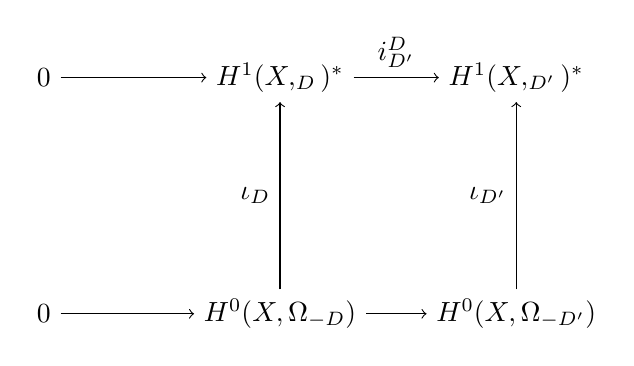
\begin{tikzpicture}[node distance=3cm, auto]
      \node (H1D) {$H^1(X, \hol_D)^\ast$};
      \node (H1D') [right of=H1D] {$H^1(X, \hol_{D'})^\ast$};
      \node (01) [left of=H1D] {0};
      \node (H0D) [below of=H1D] {$H^0(X, \Omega_{-D})$};
      \node (H0D') [right of=H0D] {$H^0(X, \Omega_{-D'})$};
      \node (02) [left of=H0D] {0};
      \draw[->] (01) to (H1D);
      \draw[->] (H1D) to node {$i_{D'}^D$} (H1D');
      \draw[->] (02) to (H0D);
      \draw[->] (H0D) to (H0D');
      \draw[->] (H0D) to node {$\iota_D$} (H1D);
      \draw[->] (H0D') to node {$\iota_{D'}$} (H1D');
    \end{tikzpicture}
  \end{center}
\end{lemma}

\begin{proof}
  Nachrechnen.\todo{Beweis das.}
\end{proof}

\begin{lemma}
  \label{lemma:urbilder}
  Sei die Notation wie in Lemma \ref{lemma:cd}. Seien weiterhin
  $\lambda \in H^1(X, \hol_D)^\ast$ und $\omega \in H^0(X,
  \Omega_{-D})$ mit $i_{D'}^D(\lambda = \iota_{D'}(\omega)$. Dann
  liegt $\omega$ bereits in $H^0(X, \Omega_{-D})$ und $\lambda =
  \iota_D (\omega)$.
\end{lemma}

\begin{proof}
  Angenommen es gelte $\omega \notin H^0(X, \Omega_{-D}) \cong
  \Omega_{-D}(X)$. Dann existierte ein $a \in X$, so dass
  $\ord_a(\omega) < D(a)$. Sei $(U_0, z)$ eine Koordinatenumgmebung
  von $a$ mit $z(a) = 0$. Auf dieser Koordinatenumgebung drücken wir
  $\omega$ durch $\omega = f \d[z]$ mit einem $f \in \mer(U_0)$
  aus. Wir können ohne Einschränkung annehmen, dass wir $U_0$ klein
  genug gewählt haben, so dass
  \begin{enumerate}
  \item $D|_{U_0 \setminus \{a\}} \equiv 0 \equiv D'|_{U_0 \setminus
      \{a\}}$ gilt und
  \item $f$ keine Null- und Polstellen auf $U_0 \setminus \{a\}$ besitzt.
  \end{enumerate}
  Nun setzen wir $U_1 := X \setminus \{a\}$, $\fu = (U_0, U_1)$ und
  $\eta = (f_0, f_1) \in C^0(\fu, \mer)$, wobei $f_0 := (zf)^{-1}$ und
  $f_1 := 0$ definiert wird. Aus $\ord_a(\omega) < D(a)$ folgte nun
  sogar, dass $\eta \in C^0(\fu, \hol_D)$ und damit sogar, dass
  \[
  \delta \eta \in Z^1(\fu, \hol) = Z^1(\fu, \hol_D) = Z^1(\fu,
  \hol_{D'})
  \]
  Bezeichnen wir mit $\xi'$ die
  Kohomologieklasse von $\delta \eta$ in $H^1(X, \hol_{D'})$ und mit
  $\xi$ die Kohomologieklasse von $\delta \eta$ in $H^1(X, \hol_D)$,
  so erhalten wir zunächst, weil $\eta \in C^0(\fu, \hol_D)$, dass
  $\xi = 0$. Nach Voraussetzung gälte nun aber
  \[
  \g{\omega}{\xi'} = \iota_{D'}(\omega)(\xi') =
  \i_{D'}^D(\lambda)(\xi') = \lambda(\xi) = 0
  \]
  Andererseits ist $\omega \eta = \left ( \frac{\d[z]}{z}, 0 \right )$
  und es folgt
  \[
  \g{\omega}{\xi'} = \res(\omega \eta) = 1
  \]
  Ein Widerspruch. Also muss $\omega \in H^0(X, \Omega_{-D})$
  gelten. Da dann $\i_{D'}^D(\lambda) = \iota_{D'}(\omega) =
  i_{D'}^D(\iota_D(\omega))$ gelten muss, folgt $\lambda =
  \iota_D(\omega)$ aus der Injektivität von $i_{D'}^D$.
\end{proof}

\begin{lemma}
  Seien $D, B \in \Div(X)$ und $X$ eine kompakte Riemannsche
  Fläche. Sei $\psi \in H^0(X, \hol_B)$. Dann induziert der
  Garbenhomomorphismus $\hol_{D-B} \xrightarrow{\psi} \hol_D$ gegeben
  durch $f \mapsto \psi f$ eine lineare Abbildung
  \[
  H^1(X, \hol_{D-B}) \ra H^1(X, \hol_D)
  \]
  und damit auch eine lineare Abbildung
  \[
  H^1(X, \hol_D)^\ast \ra H^1(X, \hol_{D-B})^\ast
  \]
  Diese bezeichnen wir auch mit $\psi$. Mit dieser Notation folgt
  $(\psi \lambda)(\xi) = \lambda(\psi \xi)$ für beliebige $\lambda \in
  H^1(X, \hol_D)^\ast$ und $\xi \in H^1(X, \hol_{D-B})$. Weiterhin
  kommutiert das folgende Diagramm
  \begin{center}
    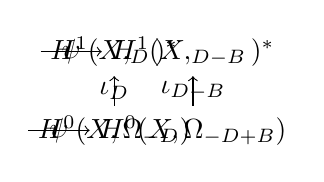
\begin{tikzpicture}
      \node (H1D) {$H^1(X, \hol_D)^\ast$};
      \node (H1B) [right of=H1D] {$H^1(X, \hol_{D-B})^\ast$};
      \node (H0D) [below of=H1D] {$H^0(X, \Omega_{-D})$};
      \node (H0B) [right of=H0D] {$H^0(X, \Omega_{-D +B})$};
      \draw[->] (H1D) to node {$\psi$} (H1B);
      \draw[->] (H0D) to node {$\psi$} (H0B);
      \draw[->] (H0D) to node {$\iota_D$} (H1D);
      \draw[->] (H0B) to node {$\iota_{D-B}$} (H1B);
    \end{tikzpicture}
  \end{center}
\end{lemma}

\begin{proof}
  Das Multiplikation mit $\psi$ ein Garbenhomomorphismus ist, ist klar
  und damit folgt die Existenz der linearen Abbildungen. Die
  Kommutativität des Diagramss erhalten wir aus der Tatsache, dass für
  beliebige $\omega \in H^0(X, \Omega_{-D})$ und $\xi \in H^1(X,
  \hol_{D-B})$ die folgende Rechnung durchführen können
  \begin{align*}
    \iota_{D-B}(\psi \omega)(\xi) = \g{\psi \omega}{\xi} = \res((\psi
    \omega) \xi) = \res(\omega (\psi \xi)) = \g{\omega}{\psi \xi} =
    \iota_D(\omega)(\psi \xi)
  \end{align*}
\end{proof}

\begin{lemma}
  \label{lemma:psi-inj}
  Falls $\psi \in H^0(X, \hol_B)$ mit $\psi \neq 0$. Dann ist $\psi:
  H^1(X, \hol_D)^\ast \ra H^1(X, \hol_{D-B})^\ast$ injektiv.
\end{lemma}

\begin{proof}
  Sei $A := (\psi) \geq -B$. Dann faktorisiert $\psi: \hol_{D-B} \ra
  \hol_D$ über $\hol_{D+A}$, d.h. das Diagramm
  \begin{center}
    \begin{tikzpicture}[node distance = 1.5cm, auto]
      \node (DB) {$\hol_{D-B}$};
      \node (D) [right of=DB] {$\hol_D$};
      \node (A) [below of=DB] {$\hol_{D+A}$};
      \draw[->] (DB) to node {$\psi$} (D);
      \draw[->] (DB) to (A);
      \draw[->, dashed] (A) to (D);
    \end{tikzpicture}
  \end{center}
  kommutiert. Weiterhin ist die Abbildung $\hol_{D+A} \ra \hol_D$ ein
  Isomorphismus, wobei die Umkehrung einfach durch Multiplikation mit
  $\psi^{-1}$ gegeben ist. Nun ist die Inklusion von $\hol_{D-B} \ra
  \hol_{D+A}$ injektiv und deshalb nach (16.8) $H^1(X, \hol_{D-B}) \ra
  H^1(X, \hol_{D+A})$ ein Epimorphismus. Also ist auch $H^1(X,
  \hol_{D-B}) \xrightarrow{\psi} H^1(X, \hol_D)$ ein Epimorphismus und
  schlussendlich die duale Abbildung injektiv. Dies zeigt die Behauptung.
\end{proof}

\begin{thm}[Der Serresche Dualitätssatz]
  Sei $D \in \Div(X)$ und $X$ eine kompakte Riemannsche Fläche. Dann
  ist $\iota_D: H^0(X, \Omega_{-D}) \ra H^1(X, \hol_D)^\ast$ ein Isomorphismus.
\end{thm}

\begin{proof}
  Aufgrund von Satz \ref{thm:iota-inj} benötigen wir nur noch die
  Surjektivität von $\iota_D$. Sei $\lambda \in H^1(X, \hol_D)^\ast$
  mit $\lambda \neq 0$ und $P \in \Div(X)$ mit $\deg P = 1$. Weiterhin
  setzen wir $D_n := D - n P$ für beliebige $n \in \N$. Als nächstes
  bezeichnen wir mit $\Lambda \subset H^1(X, \hol_{D_n})^\ast$ den
  Untervektorraum aller Linearformen der Form $\psi \lambda$, wobei
  $\psi \in H^0(X, \hol_{nP})$. Nach Lemma \ref{lemma:psi-inj} ist
  $\Lambda \cong H^0(X, \hol_{nP})$. Aus dem Satz von Riemann-Roch
  folgt damit, dass
  \[
  \dim \Lambda \geq 1 - g + n
  \]
  gilt. Aus Lemma \ref{lemma:k0} und da $\iota_{D_n}$ injektiv ist,
  erhalten wir
  \[
  \dim \im(\iota_{D_n}) = \dim H^0(X, \Omega_{-D_n}) \geq n + k_0 -
  \deg D
  \]
  Wählen wir $n > \deg D$, so erhalten wir $\deg D_n < 0$ und damit
  $H^0(X, \hol_{D_n}) = 0$. Aus dem Satz von Riemann-Roch folgt
  \[
  \dim H^1(X, \hol_{D_n})^\ast = g - 1 - \deg D_n = n + ( g - 1 -
  \deg D).
  \]
  Unter eventueller Vergrößerung von $n$ erhalten wir
  \begin{align*}
    \dim \Lambda + \dim \im(\iota_{D_n}) & \geq 1 - g + n + n + k_0 -
    \deg D \\
    & = 2 n + 1 - g + \deg D \\
    & > n + (g - 1 - \deg D) \\
    & = \dim H^1(X, \hol_{D_n})^\ast.
  \end{align*}
  Da sowohl $\Lambda$ als auch $\im(\iota_{D_n})$ Untervektorräume von
  $H^1(X, \hol_{D_n})^\ast$ sind, muss $\Lambda \cap \im(\iota_{D_n})
  \neq 0$ sein. Also existiert ein $\psi \in H^0(X, \hol_{nP})$ mit
  $\psi \neq 0$ und $\omega \in H^0(X, \Omega_{-D_n})$ mit $\psi
  \lambda = \iota_{D_n}(\omega)$. Setzen wir $A := (\psi)$, so liegt
  $\frac{1}{\psi} \in H^0(X, \hol_A)$. Zu guter Letzt erhalten wir aus
  $D' := D_n - A$, dass
  \begin{align*}
    \i_{D'}^d(\lambda) = \frac{1}{\psi} (\psi \lambda) =
    \frac{1}{\psi} \iota_{D_n}(\omega) = \iota_{D'} \left (
      \frac{1}{\psi} \omega \right )
  \end{align*}
  gilt und unter Ausnutzung von Lemma \ref{lemma:urbilder} folgt, dass
  $\omega_0 := \frac{1}{\psi} \omega \in H^0(X, \Omega_{-D})$ die
  Gleichung $\lambda = \iota_D(\omega_0)$ erfüllt.
\end{proof}

\begin{cor}
  Sei $X$ eine kompakte Riemannsche Fläche und $D \in \Div(X)$. Dann
  gilt
  \[
  \dim H^1(X, \hol_D) = \dim H^0(X, \Omega_{-D})
  \]
  Insbesondere folgt für $D = 0$
  \[
  g = \dim H^1(X, \hol) = \dim H^0(X, \Omega),
  \]
  wobei $g$ das Geschlecht von $X$ bezeichnet.
\end{cor}

%%% Local Variables: 
%%% mode: latex
%%% TeX-master: "../Bachelor"
%%% End: 

